\documentclass{article}
\usepackage{amsmath}
\usepackage{amsmath,amssymb}
\usepackage[table]{xcolor}
\usepackage{colortbl}
\usepackage{tikz}
\usepackage{pgfplots}
\usepackage[most]{tcolorbox}
\pgfplotsset{compat=1.18}

\begin{document}

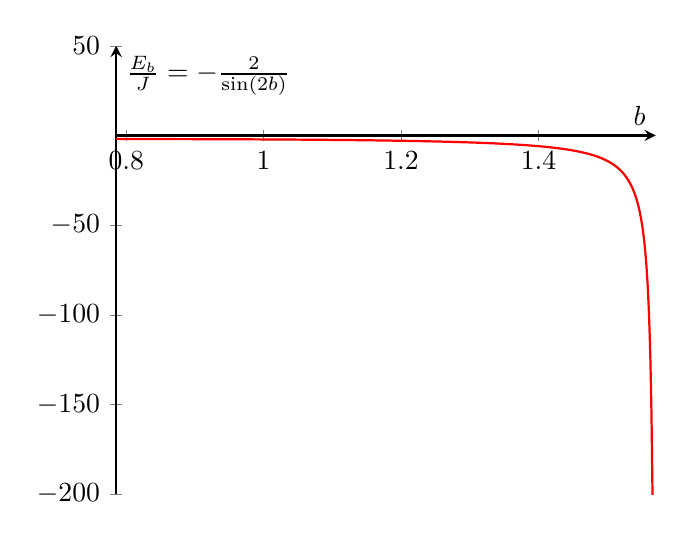
\begin{tikzpicture}
  \begin{axis}[
    axis lines=center,
    xlabel={$b$},
    ylabel={$\frac{E_b}{J}=-\frac{2}{\sin(2 b)}$},
    domain=0.7854:1.5708,
    xmin=pi/4, xmax=pi/2-0.0001,
    ymin=-200, ymax=50,
    samples=400,
    smooth,
    thick,
    ]
    \addplot [color=red, thick] {-(2)/(sin(deg(2*x)))};
  \end{axis}
\end{tikzpicture}

\end{document}